\chapter{Development of the FPGA firmware for the SFH}\label{cha:development}
The firmware developed in this thesis for the three Artix-7 FPGAs, located on the iFTDC as described in Section \ref{sec:iFTDC}, must perform several functionalities.
The main tasks of the firmware are to configure the Citiroc1A ASIC, explained in Section \ref{sec:configuration},
 communicaton with the controlling coputer via ethernet and the IPBUS protocol and a provisional readout of the time triggerd data from the Citiroc1A ASIC.
\section{The IPBUS protocol}
The IPBUS protocol used for the communication between the FPGA and the controlling computer is a simple protocol for controlling IP-aware hardware devices with a 32 bit read and write bus using UDP as the transport protocol.\autocite{IPBUS_article}
\newline
The IPBUS protocol defines a read and write command enabling successful write and read operations of a 32 bit register, with a 32 bit address in the FPGA.    
\newline
The commands can be issued on the controling computer with the $\mu$HAL library, which allowes the user to issue read and write commands with a python script and an XML file defining the address of the registers.\autocite{IPBUS_article}
\newline
The address space inside the FPGA is defined in the firmware. The address space is divided into seprate address spaces for each of the slaves by the leading bits of the address.
For some slaves, the address space is further divided into subspaces for the different registers of the slave. 
\section{Configuration of the Citiroc1A ASIC}
The configuration of the slow control and probe registers of the Citiroc1A ASIC,
 along with the verification of this configuration, is handled by two state machines. Both state machines control a single random access memory (RAM) with a depth of 64 addresses, where each address stores 32 bits of data.
The state machiens inturn are controled by the status and control register which can be written by the controlling computer via the ipbus protocol.
\subsection{Status and control register}
herre i will explain the status and control register
\subsection{Configuration state machine}
\begin{figure}[H]
    \centering
    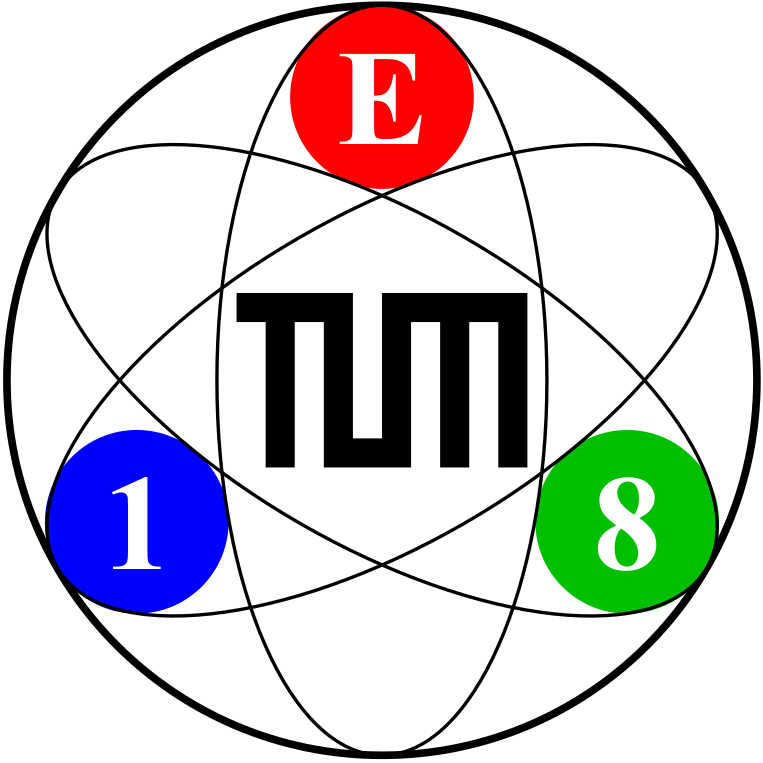
\includegraphics[width=\textwidth]{E18Logo.png}%{CONFIGSMALLdiagram2.png}
    \caption{State machine for the configuration of the Citiroc1A ASIC.}
    \label{fig:Configuration_state_machine}
\end{figure}
\subsection{Verification state machine}
\begin{figure}[H]
    \centering
    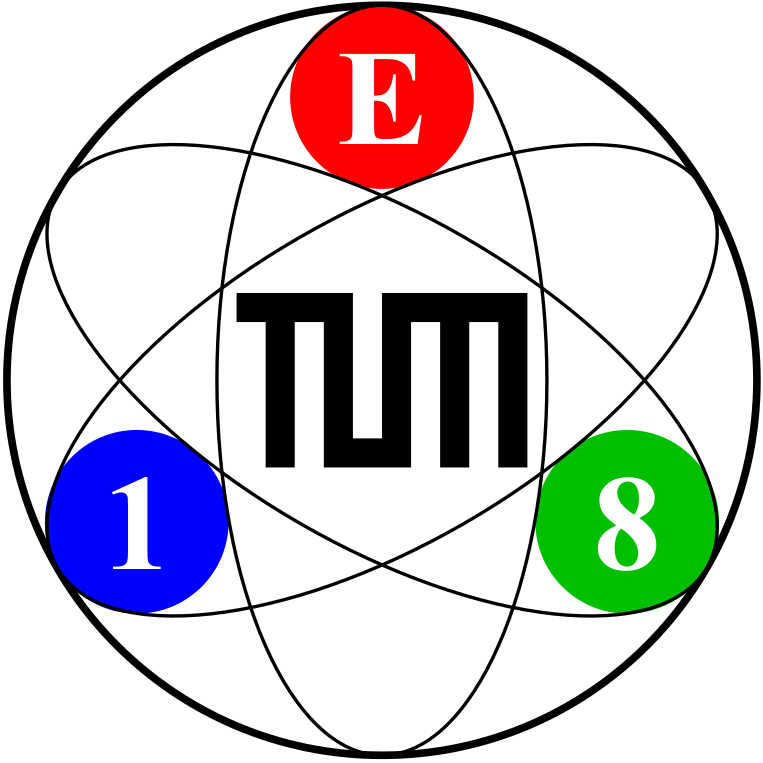
\includegraphics[width=\textwidth]{E18Logo.png}%{smallVerifacationdiagrammod.png}
    \caption{State machine for the verification of the configuration of the Citiroc1A ASIC.}
    \label{fig:Verification_state_machine}
\end{figure}
